\documentclass[border=2mm]{standalone}

\usepackage{fontspec}
\usepackage{unicode-math}

\usepackage{pgfplots}
\pgfplotsset{compat=1.18}
\usetikzlibrary{arrows.meta, 
  calc, 
  positioning, 
  decorations.pathreplacing, 
  calligraphy}

\usepackage{xcolor}
\definecolor{den-1}{HTML}{111111}   % Đen #111111
\definecolor{den-2}{HTML}{222222}   % Đen #222222
\definecolor{den-3}{HTML}{333333}   % Đen #333333
\definecolor{den-4}{HTML}{444444}   % Đen #444444
\definecolor{den-5}{HTML}{555555}   % Đen #555555
\definecolor{den-6}{HTML}{666666}   % Đen #666666

% Thiết lập vị trí đặt nhãn gốc tọa độ
\tikzset{
  >=Stealth,
  originlabel/.style={
    font=\small\sf,
    anchor=north east, % Vị trí tương đối so với gốc
    yshift=-0.1ex,     % Điều chỉnh vị trí dọc một chút
    xshift=-0.1ex      % Điều chỉnh vị trí ngang một chút
  }
}

\begin{document}

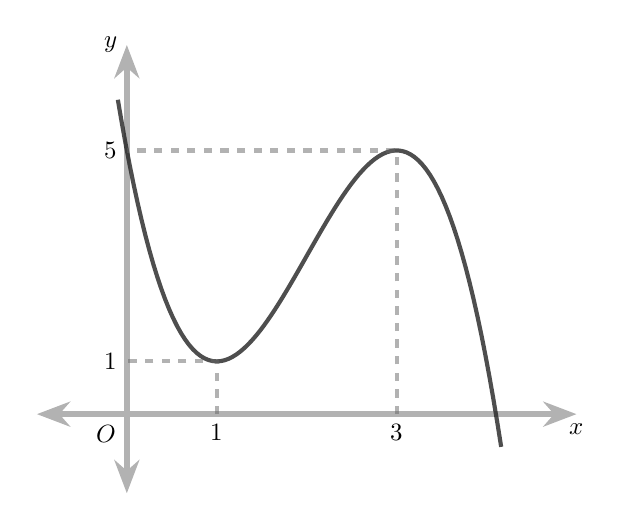
\begin{tikzpicture}
\begin{axis}[
    font=\small\sf,
    axis lines=middle,
    axis line style={<->, line width=2pt, color=den-6!50},
    xlabel=$x$, ylabel=$y$,
    xlabel style={below, font=\small\sf},
    ylabel style={left, font=\small\sf},
    domain=-.1:4.25,  
    restrict y to domain=-1:7,
    xmin=-1, xmax=5,
    ymin=-1.5, ymax=7,
    xtick={},
    xticklabels={},
    xtick style={draw=none},
    ytick={1},    
    yticklabels={}, 
    ytick style={draw=none},
    tick label style={font=\footnotesize\sf},
    clip=false,
]

\node[originlabel] at (axis cs:0,0) {$O$};

\node at (0,5) [left] {$5$};
\node at (0,1) [left] {$1$};
\node at (1,0) [below] {$1$};
\node at (3,0) [below] {$3$};

\addplot[            
      samples=100, 
      line width=1.5pt, 
      color=den-2, 
      opacity=.8
      ] 
        {-x^3+6*x^2-9*x+5};

\addplot[dashed, line width=1.5pt, color=den-6, opacity=.5] coordinates {
        (1,0)
        (1,1)
        (0,1)
        };

\addplot[dashed, line width=1.5pt, color=den-6, opacity=.5] coordinates {
        (3,0)
        (3,5)
        (0,5)
        };

\end{axis}
\end{tikzpicture}

\end{document}